% !TEX root = /media/ueslei/Ueslei/INPE/PCI/Guia_COAWST/main.tex
\chapterimage{ocean2.jpg}
\chapter{Construindo o ROMS}\index{Contruindo o ROMS}
\section{Instalando as bibliotecas do Python no computador pessoal}
\bigskip

\noindent Antes de gerar os arquivos de condições e a grade para o ROMS, é necessário instalar as bibliotecas e dependências. Nesta seção serão disponibilizados os endereços para baixá-las, bem como os comandos no terminal via \textit{apt-get}.
\bigskip

\noindent Existem duas maneiras de instalar as bibliotecas necessárias: manualmente, e através do Anaconda. Esse último é uma plataforma gratuita e de código aberto em Python e R e possui um gerenciador de pacotes chamado Conda, que facilita a instalação de bibliotecas. Neste guia, apresentarei as duas opções. Pela praticidade, sugiro instalar usando o Conda (Seção \textcolor{bleu_cite}{\ref{condasec}}), porém cuidado para conflito de versões, pois os repositórios do Conda são atualizados constantemente.
\bigskip

\begin{tcolorbox}[enhanced,
  grow to left by   = 0cm,
  grow to right by  = 0cm,
  enlarge top by    = 0cm,
  enlarge bottom by = 0cm,
  tcbox raise base,
  boxrule           = 1.0pt,
  left              = 18mm,
  colframe          = red!50!black,coltext=red!25!black,colback=red!10!white,
  overlay           = {\begin{tcbclipinterior}\fill[red!75!blue!50!white] (frame.south west)
    rectangle node[text=white,font=\sffamily\bfseries\footnotesize,rotate=0] {ATENÇÃO} ([xshift=18mm]frame.north west);\end{tcbclipinterior}}]
A construção do ROMS deverá ser feita no seu próprio computador e não mais no Kerana, como feito anteriormente com o WRF.
\end{tcolorbox}
\bigskip

\subsection{Instalação manual}\index{Instalação manual}
\bigskip
\noindent Abra o terminal, e crie uma pasta na sua \textit{home} chamada \textit{libsmodels}. Nela serão adiconados os arquivos baixados e as bibliotecas.
\bigskip

\begin{bashcode}
sudo mkdir libsmodels
\end{bashcode}
\bigskip

\noindent Caso não tenha o \textit{gfortran} e o \textit{g++} instalados, instale via \textit{apt-get}.
\bigskip
\begin{bashcode}
sudo apt-get install gfortran
sudo apt-get install g++
\end{bashcode}
\bigskip

\noindent A seguir, baixe o OpenMPI 2.0.1 (\textcolor{bleu_cite}{\textit{https://www.open-mpi.org/software/ompi/v2.0/}}), extraia o arquivo dentro da pasta \textit{libsmodels} e digite no terminal:
\bigskip

\begin{bashcode}
export F77=gfortran
export FC=gfortran
export FC=gfortran
export CC=gcc
export CXX=g++
export FFLAGS="-m64 -fdefault-integer-8"
export FCFLAGS="-m64 -fdefault-integer-8"
export CFLAGS=-m64
export CXXFLAGS=-m64
\end{bashcode}
\bigskip

\noindent Entre na pasta do OpenMPI e digite:
\bigskip

\begin{tcolorbox}[enhanced,
  grow to left by   = 0cm,
  grow to right by  = 0cm,
  enlarge top by    = 0cm,
  enlarge bottom by = 0cm,
  tcbox raise base,
  boxrule           = 1.0pt,
  left              = 18mm,
  colframe          = red!50!black,coltext=red!25!black,colback=red!10!white,
  overlay           = {\begin{tcbclipinterior}\fill[red!75!blue!50!white] (frame.south west)
    rectangle node[text=white,font=\sffamily\bfseries\footnotesize,rotate=0] {ATENÇÃO} ([xshift=18mm]frame.north west);\end{tcbclipinterior}}]
Altere o nome do computador abaixo (\textit{usuario}) pelo nome do seu computador.
\end{tcolorbox}
\bigskip

\begin{bashcode}
./configure --prefix=/home/usuario/libsmodels
sudo make
sudo make check
sudo make install
\end{bashcode}
\bigskip

\noindent Volte até a sua \textit{/home/usuario} e abra o arquivo oculto \textit{.bashrc} através do comando \textit{gedit .bashrc}e nas linhas finais do arquivo escreva:
\bigskip

\begin{bashcode}
cd /home/usuario
gedit .bashrc
export PATH=/home/usuario/libsmodels/bin:$PATH
export LD_LIBRARY_PATH=/home/usuario/libsmodels/lib:$LD_LIBRARY_PATH
export PATH=/home/usuario/libsmodels/include:$PATH
\end{bashcode}
\bigskip

\noindent Salve o arquivo e digite o comando a seguir para atualizar o terminal e aplicar as mudanças.
\bigskip

\begin{bashcode}
source .bashrc
\end{bashcode}
\bigskip

\noindent Teste a instalação do OpenMPI está correta, digite no terminal:
\bigskip

\begin{bashcode}
ompi_info -a grep 'Fort integer size'
\end{bashcode}
\bigskip

\noindent O resultado deverá ser:
\bigskip

\begin{bashcode}
Fort integer size: 8
\end{bashcode}
\bigskip

\noindent Caso não tenha instalado no seu computador, será necessário instalar o \textit{m4}, \textit{make} e \textit{perl}. Para checar se o seu computador já possui estes programas instalados:
\bigskip

\begin{bashcode}
which m4
which make
which perl
\end{bashcode}
\bigskip

\noindent Caso a resposta seja negativa, instale a partir dos comandos a seguir:
\bigskip

\begin{bashcode}
sudo apt-get install m4
sudo apt-get install make
sudo apt-get install perl
\end{bashcode}
\bigskip

\noindent Instale o \textit{szip 2.1} (\textcolor{bleu_cite}{\textit{https://www.hdfgroup.org/HDF5/release/obtain5.html}}). Baixe-o, descompacte na pasta \textit{/home/usuario/libsmodels} e entre na pasta do \textit{szip} digite:
\bigskip

\begin{bashcode}
export F77=gfortran
export FC=gfortran
export CC=gcc
export CXX=g++
export FFLAGS="-m64 -fdefault-integer-8"
export FCFLAGS="-m64 -fdefault-integer-8"
export CFLAGS=-m64
export CXXFLAGS=-m64
./configure --prefix=/home/usuario/libsmodels
sudo make
sudo make check
sudo make install
\end{bashcode}
\bigskip

\noindent Instale o \textit{zlib 1.2.8} (\textcolor{bleu_cite}{\textit{http://zlib.net/}}). Baixe-o, descompacte na pasta \textit{/home/usuario/libsmodels} e entre na pasta do \textit{zlib} digite:
\bigskip

\begin{bashcode}
export F77=gfortran
export FC=gfortran
export CC=gcc
export CXX=g++
export FFLAGS="-m64 -fdefault-integer-8"
export FCFLAGS="-m64 -fdefault-integer-8"
export CFLAGS=-m64
export CXXFLAGS=-m64
./configure --prefix=/home/usuario/libsmodels
sudo make
sudo make check
sudo make install
\end{bashcode}
\bigskip

\noindent Instale o \textit{Curl 7.50.3} (\textcolor{bleu_cite}{\textit{http://curl.haxx.se/download.html}}). Baixe-o, descompacte na pasta \textit{/home/usuario/libsmodels} e entre na pasta do \textit{Curl} digite:
\bigskip

\begin{bashcode}
export F77=gfortran
export FC=gfortran
export CC=gcc
export CXX=g++
export FFLAGS="-m64 -fdefault-integer-8"
export FCFLAGS="-m64 -fdefault-integer-8"
export CFLAGS=-m64
export CXXFLAGS=-m64
./configure --prefix=/home/usuario/libsmodels/
sudo make
sudo make check
sudo make install
\end{bashcode}
\bigskip

\noindent Instale as bibliotecas necessárias para usar o HDF5. Digite:
\bigskip

\begin{bashcode}
sudo apt-get install libgtk2.0-dev
\end{bashcode}
\bigskip

\noindent Instale o \textit{HDF5 1.8.9} (\textcolor{bleu_cite}{\textit{https://www.hdfgroup.org/HDF5/release/obtain5.html}}). Baixe-o, descompacte na pasta \textit{/home/usuario/libsmodels} e entre, via terminal, na pasta do \textit{HDF5} digite:
\bigskip

\begin{bashcode}
export FC=gfortran
export CC=gcc
export CXX=g++
export LDFLAGS=-L/home/usuario/libsmodels/lib
export CPPFLAGS=-I/home/usuario/libsmodels/include
\end{bashcode}
\bigskip

\noindent No mesmo diretório, digite:
\bigskip

\begin{bashcode}[fontsize=\footnotesize]
./configure --enable-fortran=yes --enable-fortran2003=yes --enable-cxx=yes
--with-szlib=/home/usuario/libsmodels --with-zlib=/home/usuario/libsmodels --enable-hl
--enable-shared --prefix=/home/usuario/libsmodels
\end{bashcode}
\bigskip

\noindent Complete a instalação do \textit{HDF5} com os comandos abaixo:
\bigskip

\begin{bashcode}
sudo make
sudo make check
sudo make install
\end{bashcode}
\bigskip

\noindent O próximo passo é instalar o \textit{NetCDF-C 4.4.1} (\textcolor{bleu_cite}{\textit{https://www.unidata.ucar.edu/downloads/netcdf/index.jsp}}). Baixe-o, descompacte na pasta \textit{/home/usuario/libsmodels} e na pasta do \textit{NetCDF-C} digite:
\bigskip

\begin{bashcode}[fontsize=\scriptsize]
export FC=gfortran
export CC=gcc
export CXX=g++
export LDFLAGS=-L/home/usuario/libsmodels/lib
export CPPFLAGS=-I/home/usuario/libsmodels/include
\end{bashcode}
\bigskip

\noindent Na mesma linha de comando, digite:
\bigskip

\begin{bashcode}[fontsize=\scriptsize]
./configure --prefix=/home/usuario/libsmodels --enable-netcdf4 --enable-shared --enable-dap
--with-hdf5=/home/usuario/libsmodels 
\end{bashcode}
\bigskip

\noindent Complete a instalação do \textit{NetCDF-C} com os comandos abaixo:
\bigskip

\begin{bashcode}
sudo make
sudo make check
sudo make install
\end{bashcode}
\bigskip

\noindent Instale agora o \textit{NetCDF-Fortran 4.2} (\textcolor{bleu_cite}{\textit{https://www.unidata.ucar.edu/downloads/netcdf/index.jsp}}). Baixe-o, descompacte na pasta \textit{/home/usuario/libsmodels} e na pasta do \textit{NetCDF-Fortran} digite:
\bigskip

\begin{bashcode}[fontsize=\scriptsize]
export FC=gfortran
export F77=gfortran
export CC=gcc
export CXX=g++
export LDFLAGS=-L/home/usuario/libsmodels/lib
export CPPFLAGS=-I/home/usuario/libsmodels/include
export LIBS='-lnetcdf -lhdf5 -lhdf5_hl -lz'
\end{bashcode}
\bigskip

\noindent Na mesma linha de comando, digite:
\bigskip

\begin{bashcode}
./configure --prefix=/home/usuario/libsmodels --enable-netcdf4 --enable-shared
--with-hdf5=/home/usuario/libsmodels --enable-dap
\end{bashcode}
\bigskip

\noindent Termine a instalação do \textit{NetCDF-Fortran}:
\bigskip

\begin{bashcode}
sudo make
sudo make check
sudo make install
\end{bashcode}
\bigskip

\noindent Instale o \textit{JasPer 1.900.1} (\textcolor{bleu_cite}{\textit{http://www.linuxfromscratch.org/blfs/view/svn/general/jasper.html}}). Baixe-o, descompacte na pasta \textit{/home/usuario/libsmodels} e na pasta do JasPer digite:
\bigskip

\begin{bashcode}
export FC=gfortran
export F77=gfortran
export CC=gcc
export CXX=g++
./configure --prefix=/home/usuario/libsmodels
sudo make
sudo make check
sudo make install
\end{bashcode}
\bigskip

\noindent Instale o \textit{libpng 1.6.24} (\textcolor{bleu_cite}{\textit{http://sourceforge.net/projects/libpng/?source=typ\_redirect}}). Baixe-o, descompacte na pasta \textit{/home/usuario/libsmodels} e na pasta do \textit{libpng} digite:
\bigskip

\begin{bashcode}[fontsize=\scriptsize]
export FC=gfortran
export F77=gfortran
export CC=gcc
export CXX=g++
export LDFLAGS=-L/home/usuario/libsmodels/lib
export CPPFLAGS=-I/home/usuario/libsmodels/include
export LIBS='-lz'
./configure --with-zlib=/home/usuario/libsmodels --prefix=/home/usuario/libsmodels
sudo make
sudo make check
sudo make install
\end{bashcode}
\bigskip

\noindent Instale o \textit{Udunits 2.1.24} (\textcolor{bleu_cite}{\textit{ftp://ftp.unidata.ucar.edu/pub/udunits/}}).  Baixe-o, descompacte na pasta \textit{/home/usuario/libsmodels} e entre na pasta do \textit{Udunits} digite:
\bigskip

\begin{bashcode}
export FC=gfortran
export F77=gfortran
export CC=gcc
export CXX=g++
./configure --prefix=/home/usuario/libsmodels
sudo make
sudo make check
sudo make install
\end{bashcode}
\bigskip

\noindent Instale o NetCDF4 para Python. Neste caso, baixe primeiramente o Git e use-o para baixar.
\bigskip

\begin{bashcode}
sudo apt-get install git
\end{bashcode}
\bigskip

\noindent Clone o repositório do \textit{NetCDF4-Python} com o comando:
\bigskip

\begin{bashcode}
git clone https://github.com/Unidata/netcdf4-python
\end{bashcode}
\bigskip

\noindent Entre na pasta do NetCDF4-Python e modifique o arquivo \textit{setup.cfg.template} e salve:
\bigskip

\begin{bashcode}
ncconfig    = /home/usuario/libsmodels/bin/nc-config
netCDF4_dir = /home/usuario/libsmodels
HDF5_dir    = /home/usuario/libsmodels
szip_dir    = /home/usuario/libsmodels
jpeg_dir    = /home/usuario/libsmodels
curl_dir    = /home/usuario/libsmodels
\end{bashcode}
\bigskip

\noindent Modifique o nome do arquivo \textit{setup.cfg.template} para setup.cfg:
\bigskip

\begin{bashcode}
mv setup.cfg.template setup.cfg
\end{bashcode}
\bigskip

\noindent Crie na pasta \textit{libsmodels}, as subpastas \textit{lib/python2.7/site-packages}:
\bigskip

\begin{bashcode}
mkdir lib
cd lib
mkdir python2.7
cd python2.7
mkdir site-packages
\end{bashcode}
\bigskip

\noindent Volte para a pasta principal do \textit{NetCDF4-Python} e compile:
\bigskip

\begin{bashcode}
python setup.py build
python setup.py install --prefix=/home/usario/libsmodels
\end{bashcode}
\bigskip

\noindent Caso queira conferir se a instalação ocorreu com sucesso, tente importar a biblioteca no Python. Digite no terminal:
\bigskip

\begin{bashcode}
python
import netCDF4
\end{bashcode}
\bigskip

\noindent Instale agora o \textit{mpi4py} (\textcolor{bleu_cite}{\textit{https://pypi.python.org/pypi/mpi4py)}}, extraia e digite:
\bigskip

\begin{bashcode}
python setup.py build
python setup.py install --prefix=/home/usuario/libsmodels
\end{bashcode}
\bigskip

\noindent Para testar a instalação, digite:
\bigskip

\begin{bashcode}
mpiexec -n 5 python demo/helloworld.py
\end{bashcode}
\bigskip

\noindent Instale agora o \textit{ESMF} e \textit{ESMPy} (\textcolor{bleu_cite}{\textit{https://www.earthsystemcog.org/projects/esmpy/releases}}). Primeiro digite os comandos a seguir para instalar os arquivos de bibliotecas necessárias:
\bigskip

\begin{bashcode}
sudo apt-get install python-setuptools
sudo easy_install pip
sudo pip install distribute
sudo pip install nose
\end{bashcode}
\bigskip

\noindent Dentro da pasta do ESMF, digite no terminal:
\bigskip

\begin{bashcode}[fontsize=\footnotesize]
export ESMF_F90COMPILER=gfortran
export ESMF_NETCDF_LIBS="-lnetcdff -lnetcdf"
export ESMF_DIR=/home/usuario/libsmodels/packages/esmp.ESMF_6_3_0rp1_ESMP_01/esmf
export ESMF_NETCDF="local"
export ESMF_COMPILER=gfortran
export ESMF_COMM=openmpi
export ESMF_TESTEXHAUSTIVE=on
export ESMF_TESTSHAREDOBJ=on
export ESMF_NETCDF_INCLUDE=/home/usuario/libsmodels/include
export ESMF_NETCDF_LIBPATH=/home/usuario/libsmodels/lib
export ESMF_INSTALL_PREFIX=/home/usuario/libsmodels/ESMF
make
make check
make all_tests
make install
\end{bashcode}
\bigskip

\noindent Entre na pasta \textit{scr/addon/ESMPy}:
\bigskip

\begin{bashcode}
cd src/addon/ESMPy/
\end{bashcode}
\bigskip

\noindent Na mesma linha de comando, digite:
\bigskip

\begin{bashcode}[fontsize=\footnotesize]
python setup.py build
--ESMFMKFILE=/home/usuario/libsmodels/ESMF/lib/libO/Linux.gfortran.64.openmpi.default/esmf.mk
\end{bashcode}
\bigskip

\noindent Complete a instalação:
\bigskip

\begin{bashcode}
python setup.py install --prefix=/home/usuario/libsmodels
python setup.py test
\end{bashcode}
\bigskip

\noindent Instale o Octant, utilizando o Git:
\bigskip

\begin{bashcode}
git clone https://github.com/hetland/octant
\end{bashcode}
\bigskip

\noindent Na pasta \textit{octant/external}, exclua tudo e baixe os seguintes arquivos:
\bigskip

\begin{bashcode}
rm -rf *
git clone https://github.com/sakov/gridgen-c.git
git clone https://github.com/sakov/gridutils-c
git clone https://github.com/sakov/csa-c
git clone https://github.com/sakov/nn-c
\end{bashcode}
\bigskip

\noindent Renomeie as pastas para, respectivamente: \textit{gridgen}, \textit{gridutils}, \textit{csa} e \textit{nn}. Entre na pasta \textit{nn/nn}, exporte as bibliotecas e instale o \textit{nn}:
\bigskip

\begin{bashcode}
cd nn/nn/
export FC=gfortran
export F77=gfortran
export CC=gcc
export CXX=g++
./configure --prefix=/home/usuario/libsmodels
make
make install
\end{bashcode}
\bigskip

\noindent Instale o \textit{csa} da mesma maneira que foi instalado o nn:
\bigskip

\begin{bashcode}
cd ../../csa/csa/
export FC=gfortran
export F77=gfortran
export CC=gcc
export CXX=g++
./configure --prefix=/home/usuario/libsmodels
make
make install
\end{bashcode}
\bigskip

\noindent Ainda na pasta do \textit{csa}, copie o arquivo \textit{csa.o} para a pasta \textit{/home/usuario/libsmodels/lib}:
\bigskip

\begin{bashcode}
cp csa.o /home/usuario/libsmodels/lib/l
\end{bashcode}
\bigskip

\noindent Instale o \textit{gridutils}:
\bigskip

\begin{bashcode}[fontsize=\scriptsize]
cd ../../gridutils/gridutils/
export FC=gfortran
export F77=gfortran
export CC=gcc
export CXX=g++
LDFLAGS=-L/home/usuario/libsmodels/lib
./configure --prefix=/home/usuario/libsmodels CPPFLAGS=-I/home/usuario/libsmodels/include
make
make install
\end{bashcode}
\bigskip

\noindent Instale o \textit{gridgen}:
\bigskip
\begin{bashcode}[fontsize=\scriptsize]
cd ../../gridgen/
export FC=gfortran
export F77=gfortran
export CC=gcc
export CXX=g++
LDFLAGS=-L/home/usuario/libsmodels/lib
./configure -prefix=/home/usuario/libsmodels CPPFLAGS=-I/home/usuario/libsmodels/include
\end{bashcode}
\bigskip

\noindent Abra o arquivo \textit{makefile} e altere no arquivo de acordo com o que está abaixo:
\bigskip

\begin{bashcode}
CFLAGS = -g -O2 -Wall -I/home/usuario/libsmodels/include
LDFLAGS = -L/home/usuario/libsmodels/lib
LIBS = -lgu -lm -L/home/usuario/libsmodels/lib
\end{bashcode}
\bigskip

\noindent Salve o arquivo, feche e digite no terminal:
\bigskip

\begin{bashcode}
make
make lib
make shlib
make install
\end{bashcode}
\bigskip

\noindent Dentro da pasta \textit{/home/usuario/libsmodels/octant/octant}, modifique o arquivo \textit{grid.py} como o exemplo abaixo (aproximadamente na linha 898).
\bigskip

\begin{tcolorbox}[enhanced,
  grow to left by=0cm,%   equivalent to negative mdframed 'leftmargin'
  grow to right by=0cm,%  equivalent to negative mdframed 'rightmargin'
  enlarge top by=0cm,%     equivalent to mdframed 'skipabove'
  enlarge bottom by=0cm,%  equivalent to mdframed 'skipbelow'
  tcbox raise base,
  boxrule=1.0pt,
  left=18mm,
  colframe=red!50!black,coltext=red!25!black,colback=red!10!white,
  overlay={\begin{tcbclipinterior}\fill[red!75!blue!50!white] (frame.south west)
    rectangle node[text=white,font=\sffamily\bfseries\footnotesize,rotate=0] {ATENÇÃO} ([xshift=18mm]frame.north west);\end{tcbclipinterior}}]
Observe atentamente a indentação do Python dentro dos arquivos!
\end{tcolorbox}
\bigskip


\begin{bashcode}[fontsize=\footnotesize]
self._libgridgen = np.ctypeslib.load_library('libgridgen.so', '/home/usuario/libsmodels/lib')
print octant.__path__[0]
self._libgridgen = np.ctypeslib.load_library('_gridgen', octant.__path__[0])
\end{bashcode}
\bigskip

\noindent Salve e feche o arquivo. Digite:
\bigskip

\begin{bashcode}
python setup.py build --fcompiler=gfortran
\end{bashcode}
\bigskip

\noindent Em \textit{/home/usuario/libsmodels/octant/octant}, abra o arquivo \textit{csa.py} e modifique como abaixo:
\bigskip

\begin{bashcode}
_csa = np.ctypeslib.load_library('csa.o', '/home/usuario/libsmodels/libs')
\end{bashcode}
\bigskip

\noindent Por fim, em \textit{/home/usuario/libsmodels/octant}, digite:
\bigskip

\begin{bashcode}
python setup.py install --prefix=/home/usuario/pythonmodels/octant
\end{bashcode}
\bigskip

\noindent Exporte os diretórios no \textit{.bashrc}. Lembre-se: o \textit{.bashrc} encontra-se na sua \textit{/home/usuario}.
\bigskip

\begin{bashcode}[fontsize=\scriptsize]
export PYTHONPATH=$PYTHONPATH:/home/usuario/libmodels/octant
export PYTHONPATH=$PYTHONPATH:/home/usuario/libmodels/octant/include
export PYTHONPATH=$PYTHONPATH:/home/usuario/libmodels/octant/lib/python2.7/site-packages
export PYTHONPATH=$PYTHONPATH:/home/usuario/libmodels/octant/lib
\end{bashcode}
\bigskip

\noindent Atualize o \textit{.bashrc} do terminal. Digite:
\bigskip

\begin{bashcode}
source .bashrc
\end{bashcode}
\bigskip

\subsection{Utilizando o Conda}\label{condasec}
\bigskip
\noindent O Anaconda, é uma distribuição para Python e R que fornece suporte a várias bibliotecas e pacotes utilizados neste guia, facilitando a instalação. Para isso, baixe o Anaconda (\textcolor{bleu_cite}{\textit{https://www.continuum.io/downloads}}). Para instalar basta entrar no diretório onde está o arquivo de instalação, mudar as permissões de instalação do arquivo e seguir as instruções do instalador:
\bigskip

\begin{bashcode}
 sudo chmod 770 Anaconda2.sh
 ./Anaconda2.sh
\end{bashcode}
\bigskip

\noindent A seguir, digite os seguintes comandos no terminal para instalar as bibliotecas necessários para construir um projeto no ROMS usando o Python:
\bigskip

\begin{bashcode}
conda install -c conda-forge openmpi
conda install -c anaconda gcc
conda install -c mutirri szip
conda install -c anaconda zlib
conda install -c anaconda curl
conda install -c anaconda hdf5
conda install -c conda-forge netcdf-fortran
conda install -c scitools jasper
conda install -c anaconda libpng
conda install -c conda-forge udunits
conda install -c anaconda netcdf4
conda install -c anaconda cython
conda install -c anaconda numpy
conda install -c anaconda scipy
conda install -c anaconda mpi4py
conda install -c conda-forge esmf
\end{bashcode}
\bigskip

\section{Instalando o Pyroms}\index{Instalando o Pyroms}
\bigskip

\noindent Com as bibliotecas básicas já instaladas, nesta seção será mostrado como instalar o PYROMS. Ele é uma coleção de ferramentas para ajudar com arquivos de entrada e saída do ROMS. Foi originalmente iniciado por Rob Hetland como um projeto no GoogleCode e reescrito por Frederic Castruccio. Será seguido o mesmo esquema da seção anterior, com o endereço para baixar a biblioteca e os comandos que deverão ser digitados no terminal.
\bigskip

\noindent Baixe o PyROMS dentro do seu \textit{libsmodels}:
\bigskip

\begin{bashcode}
git clone https://github.com/ESMG/pyroms.git
\end{bashcode}
\bigskip

\noindent Por fim, entre no diretório \textit{/home/usuario/libsmodels/pyroms/pyroms\_toolbox}, digite.
\bigskip

\begin{bashcode}
export FC=gfortran
export F77=gfortran
export CC=gcc
export CXX=g++
python setup.py build --fcompiler=gfortran
python setup.py install --prefix=/home/usuario/libsmodels/pyroms
\end{bashcode}
\bigskip

\noindent Instale o bathy\_smoother:
\bigskip

\begin{bashcode}
cd ../bathy_smoother/external/lp_solve_5.5/lp_solve/
sh ccc
cp bin/ux64/lp_solve /home/usuario/libsmodels/bin/
cd ../lpsolve55
sh ccc
cp bin/ux64/* /home/usuario/libsmodels/lib/
\end{bashcode}
\bigskip

\noindent Entre no diretório a seguir e abra o \textit{setup.py}:
\bigskip

\begin{bashcode}
cd ../../lp_solve_5.5/extra/Python/
gedit setup.py
\end{bashcode}
\bigskip

\noindent Mude os caminhos descritos abaixo no arquivo \textit{setup.py}. Lembre-se da indentação.
\bigskip

\begin{bashcode}[fontsize=\scriptsize]
include_dirs=['../..','/usr/include','/home/usuario/libsmodels/include'],
library_dirs=['/home/usuario/libsmodels/pyroms/lib/','/home/usuario/libsmodels/lib'],
\end{bashcode}
\bigskip

\noindent Instale:
\bigskip

\begin{bashcode}
python setup.py build
python setup.py install --prefix=/home/usuario/libsmodels/pyroms
\end{bashcode}
\bigskip

\noindent Entre no diretório do bathy\_smoother, como exemplificado abaixo e digite no terminal:
\bigskip

\begin{bashcode}
cd ../../../../../bathy_smoother/
export FC=gfortran
export F77=gfortran
export CC=gcc
export CXX=g++
python setup.py build --fcompiler=gfortran
python setup.py install --prefix=/home/usuario/libsmodels/pyroms
\end{bashcode}
\bigskip

\noindent Instale o Pyroms. Para isso use o comando para alterar o diretório:
\bigskip

\begin{bashcode}
cd ../pyroms/pyroms/
\end{bashcode}
\bigskip

\noindent Abra o arquivo \textit{hgrid.py} e mude na linha ~1028 como abaixo:
\bigskip

\begin{bashcode}[fontsize=\scriptsize]
self._libgridgen = np.ctypeslib.load_library('libgridgen.so', '/home/usuario/libsmodels/lib')
\end{bashcode}
\bigskip

\noindent Ainda no arquivo \textit{hgrid.py}, adicione a seguinte biblioteca na linha ~21:
\bigskip

\begin{bashcode}
from numpy import amin
\end{bashcode}
\bigskip

\noindent Salve, feche o \textit{hgrid.py} e digite:
\bigskip

\begin{bashcode}
cd ../
export FC=gfortran
export F77=gfortran
export CC=gcc
export CXX=g++
python setup.py build --fcompiler=gfortran
python setup.py install --prefix=/home/usuario/libsmodels/pyroms
\end{bashcode}
\bigskip

\noindent Coloque os caminhos no seu \textit{.bashrc}:
\bigskip

\begin{bashcode}[fontsize=\tiny]
export PYTHONPATH=$PYTHONPATH:/home/usuario/libsmodels/pyroms/lib/python2.7/site-packages
export PYTHONPATH=$PYTHONPATH:/home/usuario/libsmodels/pyroms/lib/python2.7/site-packages
export PYTHONPATH=$PYTHONPATH:/home/usuario/libsmodels/pyroms/lib/python2.7/site-packages
export PYTHONPATH=$PYTHONPATH:/home/usuario/libsmodels/pyroms/lib
export PYTHONPATH=$PYTHONPATH:/home/usuario/libsmodels/pyroms/lib/python2.7/site-packages/pyroms_toolbox/Grid_HYCOM
export PYTHONPATH=$PYTHONPATH:/home/usuario/libsmodels/pyroms/examples
\end{bashcode}
\bigskip

\noindent Atualize o \textit{.bashrc}:
\bigskip
\begin{bashcode}
source .bashrc
\end{bashcode}
\bigskip

\noindent Vá até \textit{/home/usuario/libsmodels/pyroms/lib/python2.7/site-packages/bathy\_smoother/} e apague o arquivo lpsolve55.so.
\bigskip

\noindent Por fim, vá na pasta agora do \textit{pyroms\_toolbox/} e abra o \textit{\_\_init\_\_.py} e comente a linha que importa \textit{from move\_river\_t import move\_river\_t} (~linha 51), depois na pasta \textit{Grid\_HYCOM} no arquivo \textit{flood\_fast.py} e comente na linha ~9 o \textit{import creep}.
\bigskip

\noindent Salve e tente importar o pyroms\_toolbox:
\bigskip

\begin{bashcode}
python
import pyroms_toolbox
\end{bashcode}
\bigskip 

\section{O model2roms}\index{O model2roms}\label{model2romssec}
\bigskip

\noindent Nessa seção será mostrado como instalar o model2roms, programa utilizado para gerar as condições e grade do ROMS. O \textit{model2roms} é composto por vários scripts para criação dos arquivos de entrada do ROMS. Foi originalmente iniciado por Trond Kristiansen (\textcolor{bleu_cite}{\cite{Trond2019}}) e foi adaptado para as necessidades do LOA-INPE. Será seguido o mesmo esquema da seção anterior, com o endereço para baixar a biblioteca e os comandos que deverão ser digitados no terminal.
\bigskip

\noindent Para baixar o \textit{model2roms}, entre na \textit{home} do seu computador e baixe o \textit{model2roms} utilizando o Github:
\bigskip

\begin{bashcode}
cd /home/usuario
git clone https://github.com/usutil/model2roms
\end{bashcode}
\bigskip

\noindent Altere o nome da pasta de \textit{model2roms-master} para \textit{model2roms}:
\bigskip

\begin{bashcode}
mv model2roms-master model2roms
\end{bashcode}
\bigskip

\subsection{Introdução sobre a grade do ROMS}\index{Gerar a grade do ROMS}
\bigskip

\noindent Para gerar a grade do ROMS, usaremos o script \textit{make\_roms\_grid.py}, localizado no diretório \textit{model2roms/grid}.  O script oferece suporte aos dados do SRTM30\_plus (\cite{Becker2009}), porém, para fins práticos, exemplificaremos apenas os dados do ETOPO1, que será discutido na próxima subseção.
\bigskip

\noindent Caso seja necessário, instale o basemap para utilizar o script:
\bigskip

\begin{bashcode}
conda install -c anaconda basemap
\end{bashcode}
\bigskip

\subsection{O ETOPO1 1 Arc-Minute Global Relief Model}\index{O ETOPO1 1 Arc-Minute Global Relief Model}
\bigskip

\noindent O ETOPO1 (\cite{Amante2009}; Figura \textcolor{bleu_cite}{\ref{etopo1}}) é produzido pelo National Geophysical Data Center e fornece duas camadas de informações de relevo. As camadas incluem batimetria sobre os oceanos e alguns dos principais lagos da Terra. A topografia terrestre e a batimetria oceânica baseiam-se na topografia SRTM30 e através de vários cruzeiros batimétricos. 
\bigskip

\noindent Acesse o site: \textcolor{bleu_cite}{\textit{https://www.ngdc.noaa.gov/mgg/global/global.html}}
\bigskip
   
\begin{figure}[H]
    \centering
    \captionsetup{justification=centering}
    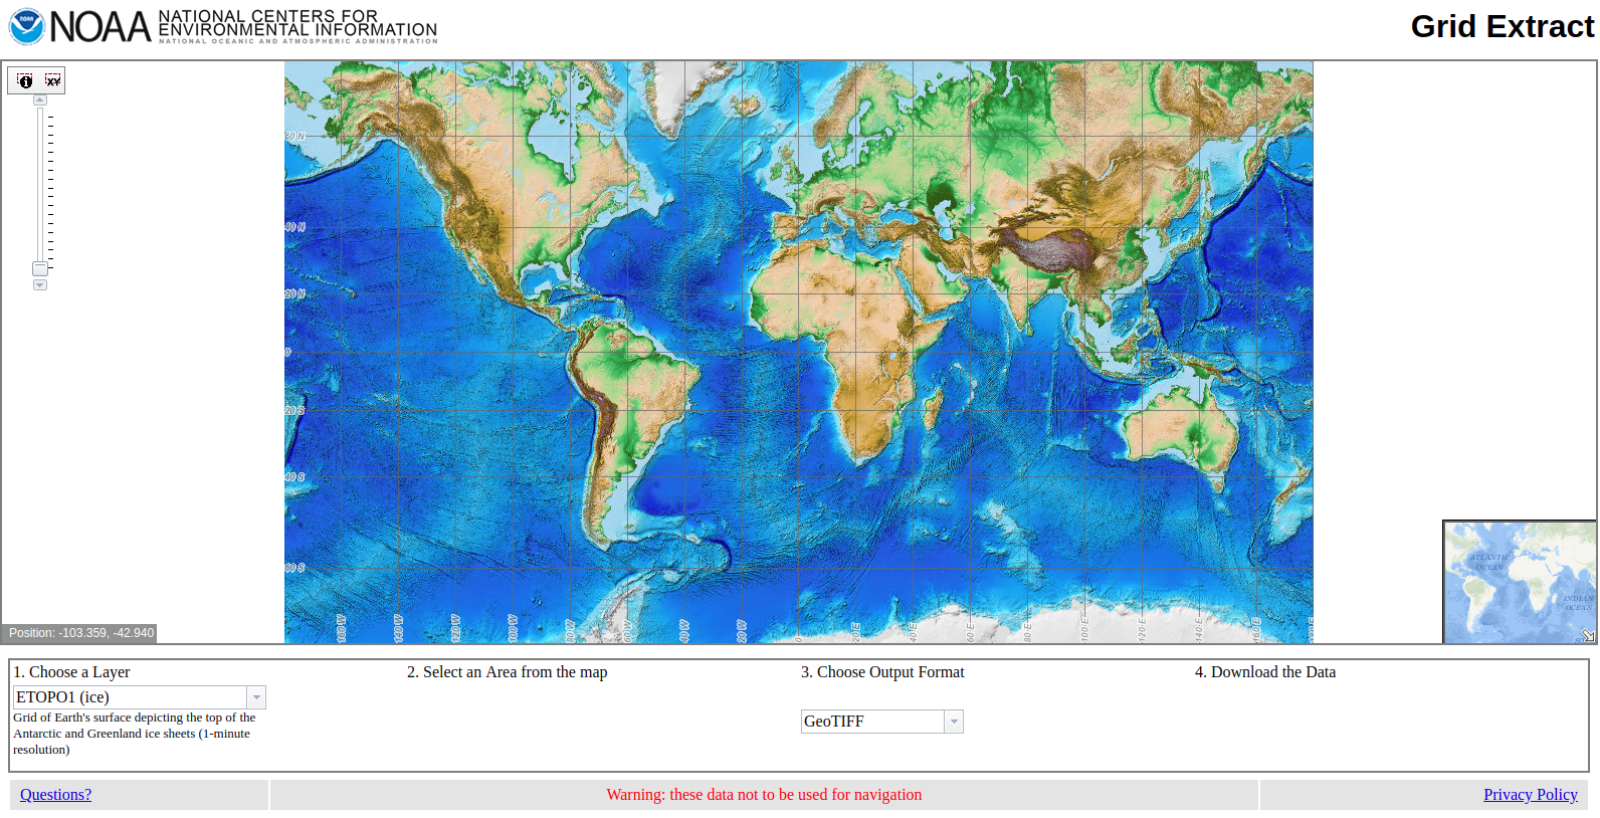
\includegraphics[width=0.85\textwidth]{etopo1.png}
    \caption{Apresentação do site do ETOPO1.}
    \label{etopo1}
\end{figure}
\bigskip

\noindent Delimite no mapa do site do ETOPO1 a sua área de interesse e baixe os dados no formato NetCDF. 
\bigskip

\begin{tcolorbox}[enhanced,
    grow to left by   = 0cm,
    grow to right by  = 0cm,
    enlarge top by    = 0cm,
    enlarge bottom by = 0cm,
    tcbox raise base,
    boxrule           = 1.0pt,
    left              = 18mm,
    colframe          = red!50!black,coltext=red!25!black,colback=red!10!white,
    overlay           = {\begin{tcbclipinterior}\fill[red!75!blue!50!white] (frame.south west)
      rectangle node[text=white,font=\sffamily\bfseries\footnotesize,rotate=0] {ATENÇÃO} ([xshift=18mm]frame.north west);\end{tcbclipinterior}}]
  O script \textit{make\_roms\_grid.py} não permite a seleção dos limites de latitude e longitude da grade, portanto, ao baixar os dados do ETOPO1, seja o mais preciso possível no recorte da sua área.
\end{tcolorbox}
\bigskip

\subsubsection{Gerando a grade do ROMS}\index{Gerando a grade do ROMS}

\noindent Entre no diretório do \textit{model2roms} e procure pela subpasta \textit{grid}. Abra o script \textit{make\_roms\_grid.py}.
\bigskip

\begin{bashcode}
cd /home/usuario/model2roms/grid
gedit make_roms_grid.py
\end{bashcode}
\bigskip

\noindent Conforme a Figura \textcolor{bleu_cite}{\ref{fazgrade}}, as variáveis que serão modificadas são:
\bigskip

\begin{itemize}
\item \textbf{grd\_name}: Nome da grade;
\item \textbf{grd\_final}: O nome do arquivo NetCDF da grade;
\item \textbf{etopo1\_dir}: O diretório onde está localizado o arquivo NetCDF do ETOPO1;
\item\textbf{srtm\_dir}: O diretório onde está localizado o arquivo NetCDF do SRTM\_30\_PLUS; 
\item \textbf{hmin}: Valor mínimo de h;
\item \textbf{theta\_b}: Parâmetro de controle das coordenadas próximas ao fundo oceânico;
\item \textbf{theta\_s}: Parâmetro de controle das coordenadas próximas à superfície;
\item \textbf{Tcline}: Profundidade crítica, em metros, controlando o alongamento das coordenadas seguidoras do terreno. Pode ser interpretado como a largura da superfície onde a resolução vertical é melhor;
\item \textbf{N}: Número de camadas Sigma;
\item \textbf{rmax}: Fator de suavização da topografia;
\item \textbf{intrp\_method}: Método de interpolação da grade: Interpolação linear (\textit{linear}) ou por Vizinho Próximo (\textit{nn});
\item \textbf{grid\_resolution}: Resolução da grade;
\item\textbf{max\_depth}: Profundidade máxima da grade.
\end{itemize}
\bigskip

\begin{tcolorbox}[enhanced,
    grow to left by   = 0cm,
    grow to right by  = 0cm,
    enlarge top by    = 0cm,
    enlarge bottom by = 0cm,
    tcbox raise base,
    boxrule           = 1.0pt,
    left              = 18mm,
    colframe          = red!50!black,coltext=red!25!black,colback=red!10!white,
    overlay           = {\begin{tcbclipinterior}\fill[red!75!blue!50!white] (frame.south west)
      rectangle node[text=white,font=\sffamily\bfseries\footnotesize,rotate=0] {ATENÇÃO} ([xshift=18mm]frame.north west);\end{tcbclipinterior}}]
  Em \textit{grid\_resolution}, é necessário colocar o numerador para fazer o cálculo do ETOPO1. Por exemplo: como o ETOPO1 possui 1/60° de resolução espacial, caso a resolução espacial escolhida seja de 1/12°, o valor de \textit{grid\_resolution} será 5, pois 5/60° será 1/12°.
\end{tcolorbox}
\bigskip

\begin{tcolorbox}[enhanced,
    grow to left by   = 0cm,
    grow to right by  = 0cm,
    enlarge top by    = 0cm,
    enlarge bottom by = 0cm,
    tcbox raise base,
    boxrule           = 1.0pt,
    left              = 18mm,
    colframe          = red!50!black,coltext=red!25!black,colback=red!10!white,
    overlay           = {\begin{tcbclipinterior}\fill[red!75!blue!50!white] (frame.south west)
      rectangle node[text=white,font=\sffamily\bfseries\footnotesize,rotate=0] {ATENÇÃO} ([xshift=18mm]frame.north west);\end{tcbclipinterior}}]
  Como não utilizaremos os dados do SRTM\_30\_PLUS, a variável \textit{srtm\_dir} não precisa ser modificada.
\end{tcolorbox}
\bigskip

\begin{figure}[H]
    \centering
    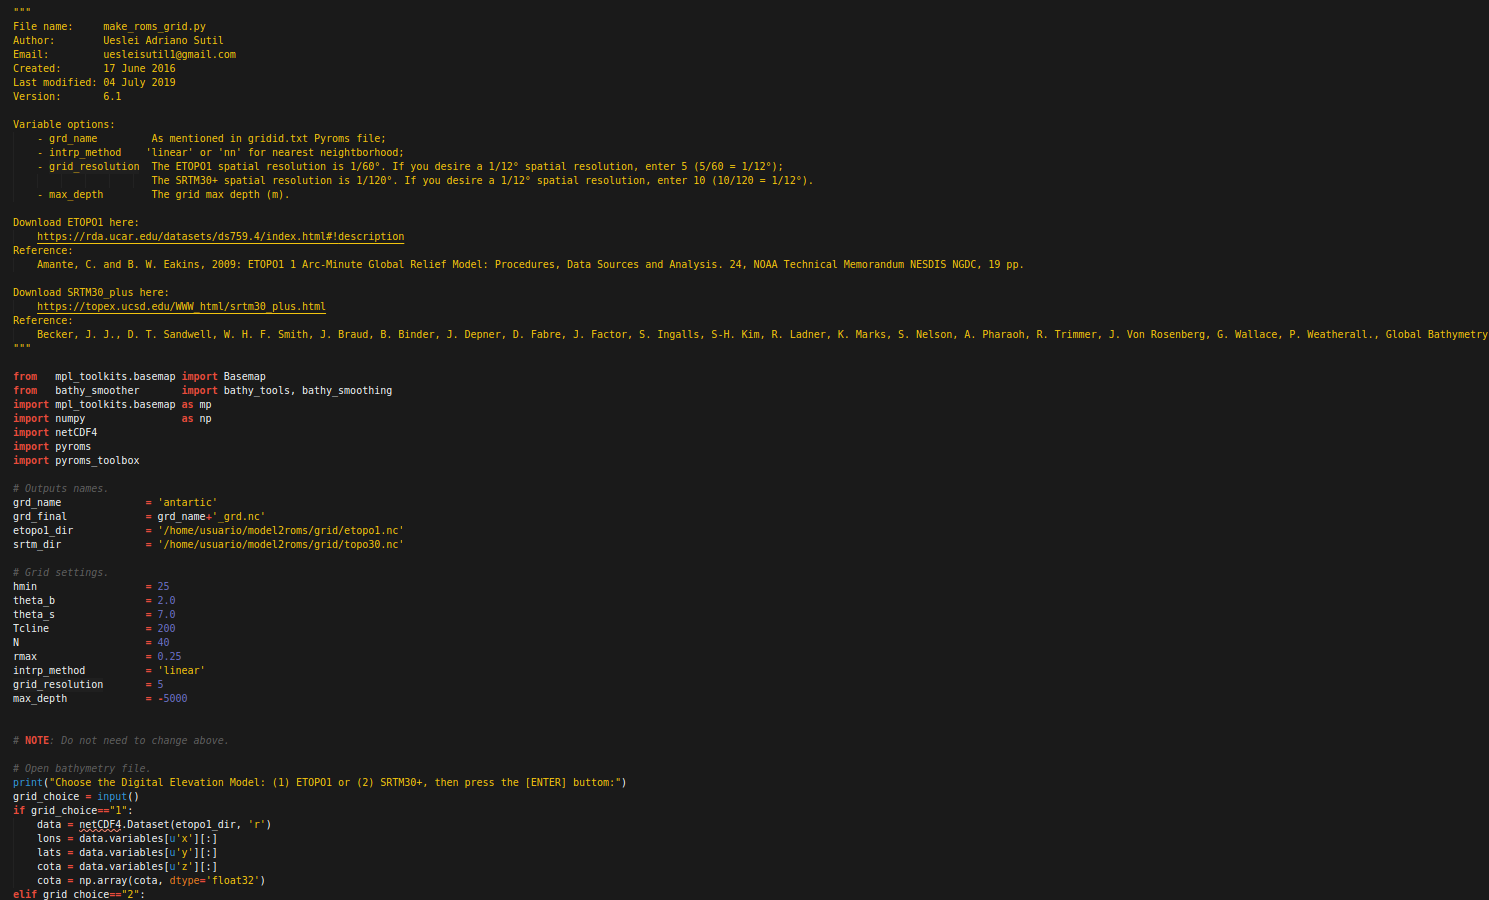
\includegraphics[width=1\textwidth]{makegrid.png}
    \caption{Captura de tela do script \textit{make\_grid.py}, que se encontra dentro da pasta \textit{model2roms/grid}.}
    \label{fazgrade}
\end{figure}
\bigskip

\noindent Após realizar as modificações, basta apenas executar o script. Digite:
\bigskip

\begin{bashcode}
ipython make_roms_grid.py --pylab
\end{bashcode}
\bigskip

\subsection{Introdução sobre as condições do ROMS}\index{Introdução sobre as condições do ROMS}
\bigskip

\noindent Utilizaremos o \textit{model2roms} para gerar as condições do ROMS. A toolbox oferece suporte aos dados do GLORYS12V1 (\cite{Fernandez2018}) e SODA3 \cite{Carton2018}), porém, utilizaremos apenas o GLORYS12V1 como exemplo.

\subsection{O Global Ocean Physics Reanalysis (GLORYS)}\index{O Global Ocean Physics Reanalysis (GLORYS)}
\bigskip

\noindent  O GLORYS é uma reanálise global do oceano com resolução espacial de 1/12°, resulção temporal diária ou mensal e 50 níveis verticais. Ele é baseado no atual sistema CMEMS de previsão global do tempo e é forçado pelo ERA-Interim do ECMWF a partir do modelo NEMO. É utilizado um filtro de Kalman de ordem reduzida para assimilar os dados de altimetria do mar, temperatura da superfície do mar, concentração de gelo marinho obtidos a partir de sensoriamento remoto e os dados \textit{in situ} de perfis verticais de temperatura e salinidade. Além disso, um esquema 3D-VAR fornece uma correção para os desvios de de temperatura e salinidade. 
\bigskip

\noindent O GLORYS pode ser baixado no site: \textcolor{bleu_cite}{\textit{http://marine.copernicus.eu/services-portfolio/access-to-products/?option=com\_csw\&view=details\&product\_id=GLOBAL\_REANALYSIS\_PHY\_001\_030}}
\bigskip

\noindent Ao tentar baixar, o site avisará que será necessário criar uma conta no Copernicus. Faça o cadastro e escolha o conjunto de dados diários do GLORYS, conforme a Figura \textcolor{bleu_cite}{\ref{glorys1}}.
\bigskip

\begin{figure}[H]
    \centering
    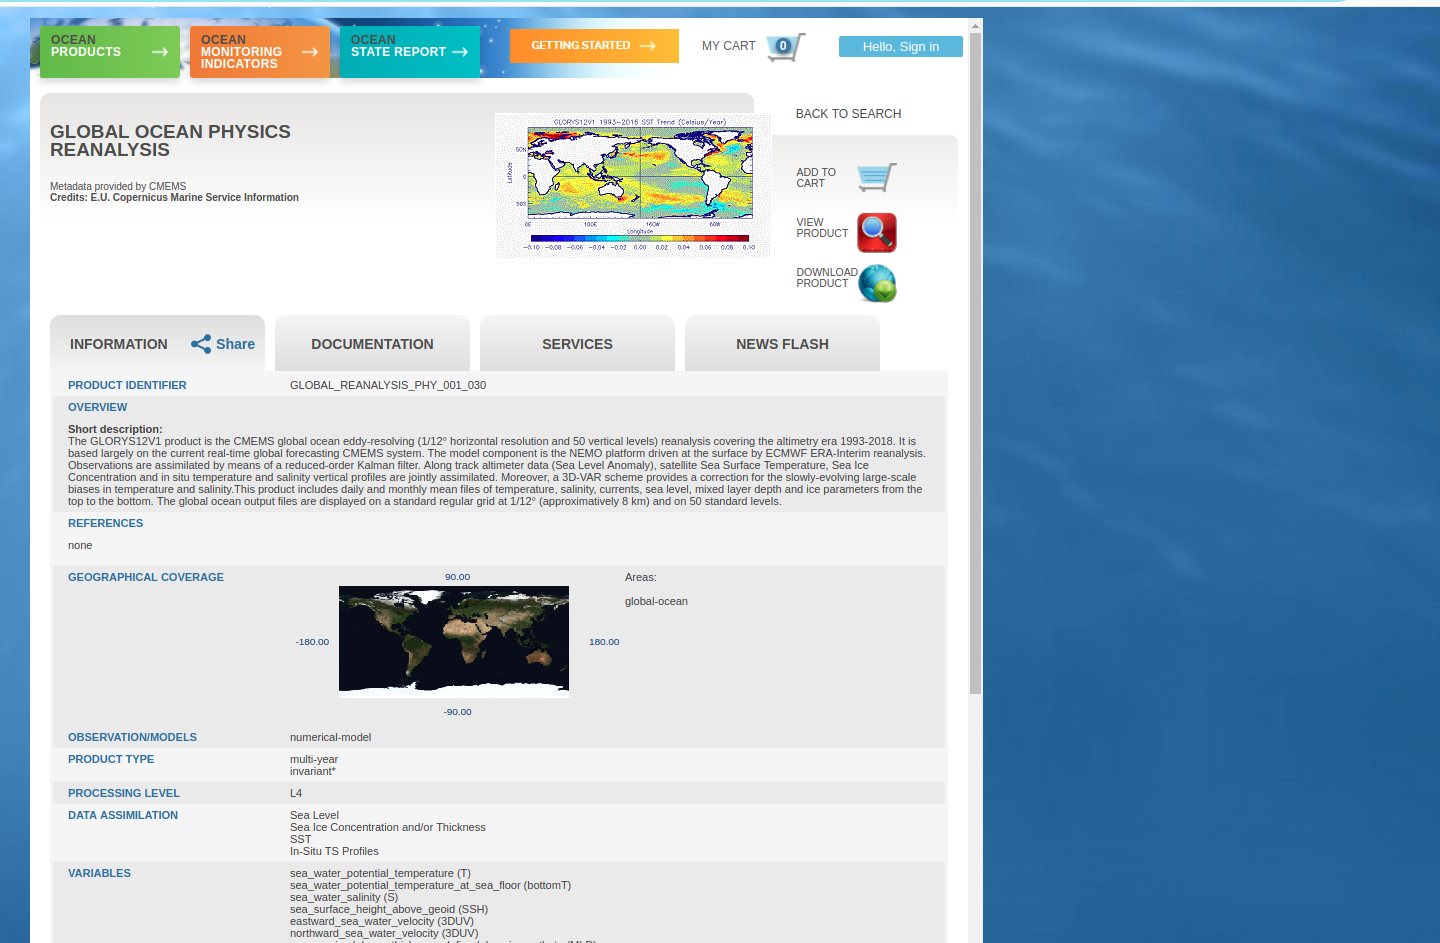
\includegraphics[width=0.7\textwidth]{glorys1.png}
    \caption{Captura de tela do site do GLORYS.}
    \label{glorys1}
\end{figure}
\bigskip

\noindent Clique em \textit{Dowload product} e, na próxima página (Figura \textcolor{bleu_cite}{\ref{glorys2}}), selecione a área conforme os limites de latitude e longitude da grade escolhida. Também escolha o período dos dados que serão baixados e caso pretenda utilizar o modelo de gelo marinho no ROMS, selecione todas as variáveis, com excessão de: 
\bigskip
\begin{itemize}
    \item \textit{ bottomT - Sea floor potential temperature};
    \item \textit{mlotst - Density ocean mixed layer thickness}.
\end{itemize}
\bigskip

\noindent Caso escolha não utilizar o modelo de gelo marinho, não selecione as variáveis:
\bigskip

\begin{itemize}
    \item \textit{siconc - Ice concentration};
    \item \textit{sithick - Sea ice thickness};
    \item \textit{usi - Sea ice eastward velocity};
    \item \textit{vsi - Sea ice northward velocity}.
\end{itemize}
\bigskip

\begin{figure}[H]
    \centering
    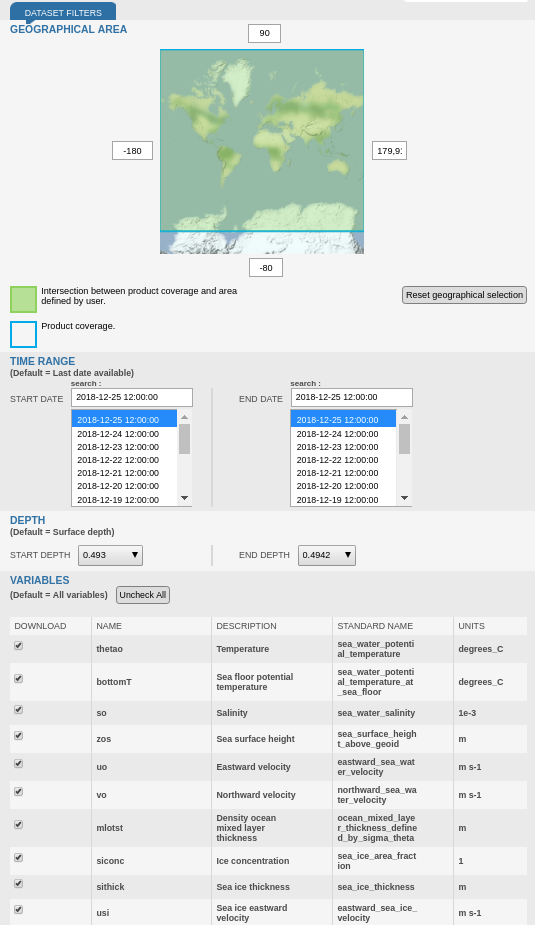
\includegraphics[width=0.6\textwidth]{glorys2.png}
    \caption{Captura de tela do site do GLORYS.}
    \label{glorys2}
\end{figure}
\bigskip

\noindent O servidor do Copernicus libera para download arquivos com no máximo 1024 mb. Caso o período selecionado apresente um tamanho de arquivo maior, como por exemplo na Figura \textcolor{bleu_cite}{\ref{glorys3}}, será necessário retornar ao passo anterior e particionar os arquivos em datas menores ou então baixar o arquivo completo clicando em \textit{FTP ACCESS} (Figura \textcolor{bleu_cite}{\ref{glorys3}})
\bigskip

\begin{figure}[H]
    \centering
    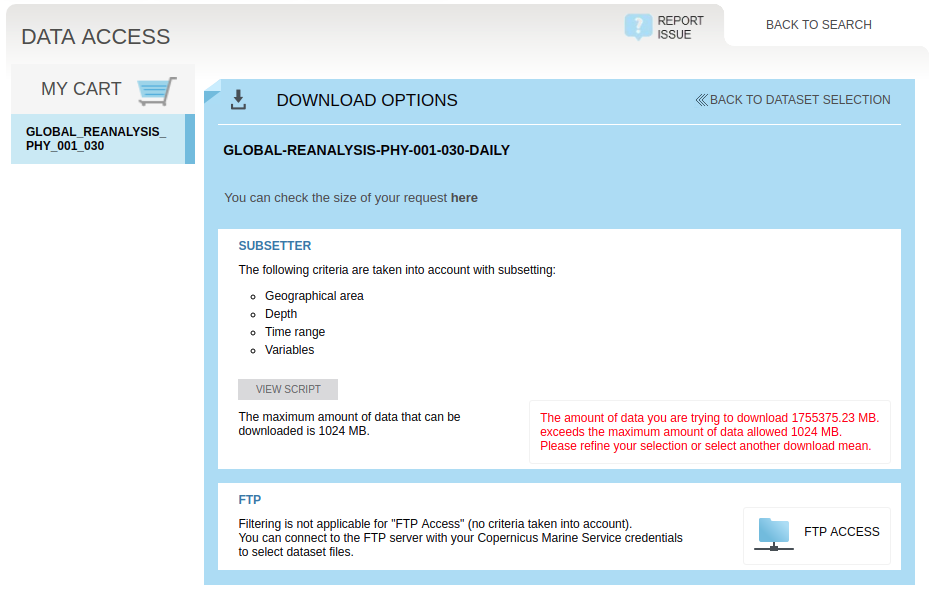
\includegraphics[width=0.6\textwidth]{glorys3.png}
    \caption{Mensagem de erro ao tentar realizar o \textit{download} de um arquivo maior que 1024 mb.}
    \label{glorys3}
\end{figure}
\bigskip


\noindent Caso opte particionar as datas ou baixar os arquivos por \textit{FTP}, será necessário criar um novo arquivo com todas as datas escolhidas. Neste caso, é necessário utilizar o \textit{Climate Data Operators} (CDO). 
\bigskip

\noindent Existem duas maneiras de  instalar o CDO: pelo \textit{Conda} ou por \textit{apt-get}.
\bigskip

\noindent Pelo \textit{Conda}, digite:
\bigskip

\begin{bashcode}
conda install -c conda-forge cdo
\end{bashcode}
\bigskip

\noindent Por \textit{apt-get}:
\bigskip

\begin{bashcode}
sudo apt-get install cdo
\end{bashcode}
\bigskip

\noindent Após a instalação, entre no diretório onde estão localizados todos os arquivos do GLORYS e digite:
\bigskip

\begin{bashcode}
cdo cat glorys* glorys.nc
\end{bashcode}
\bigskip

\noindent Onde: 
\bigskip

\begin{itemize}
    \item  \textit{cdo} significa o comando do programa;
    \item \textit{cat} a concatenação de todos os arquivos;
    \item \textit{glorys*} que serão concatenados todos os arquvis chamados \textit{glorys} dentro da pasta; 
    \item \textit{glorys.nc} o arquivo final criado pela concatenação do \textit{CDO}.
\end{itemize}

\begin{tcolorbox}[enhanced,
    grow to left by   = 0cm,
    grow to right by  = 0cm,
    enlarge top by    = 0cm,
    enlarge bottom by = 0cm,
    tcbox raise base,
    boxrule           = 1.0pt,
    left              = 18mm,
    colframe          = red!50!black,coltext=red!25!black,colback=red!10!white,
    overlay           = {\begin{tcbclipinterior}\fill[red!75!blue!50!white] (frame.south west)
      rectangle node[text=white,font=\sffamily\bfseries\footnotesize,rotate=0] {ATENÇÃO} ([xshift=18mm]frame.north west);\end{tcbclipinterior}}]
  Para facilitar os próximos passos, coloque o arquivo do GLORYS dentro do diretório \textit{/home/usuario/model2roms/input}
\end{tcolorbox}

\subsection{Gerando as condições do ROMS}\index{Gerando as condições do ROMS}
\bigskip

\noindent Ao abrir a pasta do \textit{model2roms} é possível observar diversos scripts. Começaremos com o script o \textit{compile.py}, que compilará diversos arquivos em linguagem Fortran90 para Python.
\bigskip

\noindent Compile os arquivos com o comando:
\bigskip

\begin{bashcode}
ipython compile.py --pylab
\end{bashcode}
\bigskip

\noindent Caso o nome do seu arquivo do \textit{GLORYS} seja diferente de \textit{glorys.nc}, abra o script \textit{forcingFilenames.py} (Figura \textcolor{bleu_cite}{\ref{forcingfilename}}) e na linha 15, altere \textit{'glorys.nc'} para o nome do arquivo criado.
\bigskip

\begin{bashcode}
cd /home/usuario/model2roms
gedit forcingFilenames.py
\end{bashcode}
\bigskip

\begin{figure}[H]
    \centering
    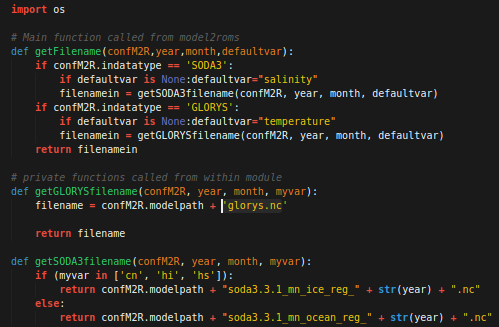
\includegraphics[width=0.6\textwidth]{forcingfilename.png}
    \caption{Captura de tela do script \textit{forcingFilename.py}.}
    \label{forcingfilename}
\end{figure}
\bigskip

\noindent Abra o arquivo \textit{configM2R.py} e, na linha 16 (Figura \textcolor{bleu_cite}{\ref{abrev}}), altere a abreviação \textit{SuaAbreviaçãoAqui} da definição \textit{defineabbreviation} para o nome de sua escolha.
\bigskip

\begin{figure}[H]
    \centering
    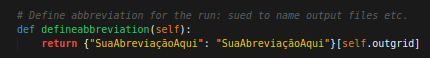
\includegraphics[width=0.6\textwidth]{abrevi.png}
    \caption{Captura de tela da definição \textit{defineabbreviation} no script \textit{configM2R.py}.}
    \label{abrev}
\end{figure}
\bigskip

\noindent Na linha 63 (Figura \textcolor{bleu_cite}{\ref{gradediretoriom2r}}), altere o diretório da grade \textit{Minha\_Grade.nc} para o diretório da grade escolhida e a abreviação \textit{SuaAbreviaçãoAqui} pelo nome escolhido no passo anterior.
\bigskip

\begin{figure}[H]
    \centering
    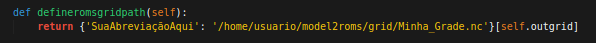
\includegraphics[width=0.6\textwidth]{m2rgriddir.png}
    \caption{Captura de tela do script \textit{configM2R.py}.}
    \label{gradediretoriom2r}
\end{figure}
\bigskip

\noindent Na linha 67 (Figura \textcolor{bleu_cite}{\ref{glorysdirm2r}}), altere o diretório do arquivo do \textit{GLORYS} para o caminho escolhido.
\bigskip


\begin{figure}[H]
    \centering
    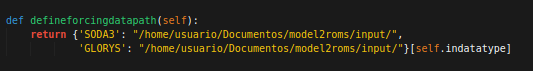
\includegraphics[width=0.6\textwidth]{glorysdirm2r.png}
    \caption{Captura de tela do script \textit{configM2R.py}.}
    \label{glorysdirm2r}
\end{figure}
\bigskip

\noindent A partir da linha 76 (Figura \textcolor{bleu_cite}{\ref{m2roptions}}), modifique de acordo com o seu projeto:
\bigskip

\begin{itemize}
    \item \textbf{self.compileall}: \textit{True} caso deseje que os arquivos em Fortran sejam recompilados cada vez que o \textit{model2roms} for executado;
    \item \textbf{self.createoceanforcing}: \textit{True} para criar as forçantes oceânicas;
    \item \textbf{self.createatmosforcing}: \textit{True} para criar as forçantes atmosféricas. \textbf{Atualmente esta função encontra-se indisponível};
    \item \textbf{self.writeice}: \textit{True} para criar as forçantes de gelo marinho.
    \item \textbf{self.set2DvarsToZero}: Cria os arquivos de gelo e altura do nível do mar com valores zerados. Como o GLORYS possui esses valores, é recomendado deixar \textit{False};
    \item \textbf{self.useesmf}: \textit{True} para usar o \textit{ESMF} para interpolar os dados do GLORYS para a grade do ROMS;
    \item \textbf{self.usefilter}: \textit{True} para aplicar um filtro para suavizar os campos 2D.
    \item \textbf{self.myformat}: O formato para escrever os arquivos de entrada do ROMS. Por padrão \textit{NETCDF};
    \item \textbf{self.timefrequencyofinputdata}: A frequência dos dados de entrada. No caso do GLORYS, escrever \textit{'day'};
    \item \textbf{self.indatatype}: O nome do dado utilizado para gerar as condições. \textit{'GLORYS} ou \textit{SODA3};
    \item \textbf{self.authorname}: O nome do usuário que está utilizando o \textit{model2roms};
    \item \textbf{self.authoremail}: O email do usuário que está utilizando o \textit{model2roms};
    \item \textbf{self.ingridtype}: Interpolará a grade do GLORYS, que é em coordenada \textit{'ZLEVEL'};
    \item \textbf{self.grdtype}: O tipo de grade do GLORYS, que é \textit{'regular'};
    \item \textbf{self.lonname}: O nome da variável de longitude do GLORYS, que é \textit{'longitude'};
    \item \textbf{self.latname}: O nome da variável de latitude do GLORYS, que é \textit{'latitude'};
    \item \textbf{self.depthname}: O nome da variável de profundidade do GLORYS, que é \textit{'depth'};
    \item \textbf{self.lonname\_u}: O nome da variável de longitude em U do GLORYS, que é \textit{'longitude'};
    \item \textbf{self.latname\_u}: O nome da variável de latitude em U do GLORYS, que é \textit{'latitude'};
    \item \textbf{self.lonname\_v}: O nome da variável de longitude em V do GLORYS, que é \textit{'longitude'};
    \item \textbf{self.latname\_v}: O nome da variável de latitude em V do GLORYS, que é \textit{'latitude'};
    \item \textbf{self.timename}: O nome da variável de tempo do GLORYS, que é \textit{'time'};
    \item \textbf{self.realm}: O ambiente em que está sendo executado o 'textit{model2roms}, neste caso, \textit{'ocean'};
    \item \textbf{self.fillvaluein}: O valor de \textit{fillvalue} do arquivo NetCDF. Por definição, \textit{-1.e20};
    \item \textbf{self.outgrid}: O nome da abreviação utilizada na definição \textit{defineabbreviation};
    \item \textbf{self.outgridtype}: Se \textit{"ROMS"}, criará as saídas no formato padrão do ROMS;
    \item \textbf{self.nlevels}: O número de níveis verticais da grade. Deverá ser o mesmo que o escolhido no script \textit{make\_roms\_grid.py};
    \item \textbf{self.vstretching}: Deverá ser o mesmo que o escolhido no script \textit{make\_roms\_grid.py};
    \item \textbf{self.vtransform}: Deverá ser o mesmo que o escolhido no script \textit{make\_roms\_grid.py};
    \item \textbf{self.theta\_s}: Deverá ser o mesmo que o escolhido no script \textit{make\_roms\_grid.py};
    \item \textbf{self.theta\_b}: Deverá ser o mesmo que o escolhido no script \textit{make\_roms\_grid.py}.
    \item \textbf{self.tcline}: Deverá ser o mesmo que o escolhido no script \textit{make\_roms\_grid.py}.   
    \item \textbf{self.hc}: Deverá ser o mesmo que o escolhido no script \textit{make\_roms\_grid.py}.
    \item \textbf{self.start\_year}: O ano inicial dos dados do GLORYS;
    \item \textbf{self.end\_year}: O ano final dos dados do GLORYS;  
    \item \textbf{self.start\_month}: O mês inicial dos dados do GLORYS;  
    \item \textbf{self.end\_month}: O mês final dos dados do GLORYS;  
    \item \textbf{self.start\_day}: O dia inicial dos dados do GLORYS;  
    \item \textbf{self.end\_day}: O dia final dos dados do GLORYS;    
\end{itemize}
\bigskip

\begin{figure}[H]
    \centering
    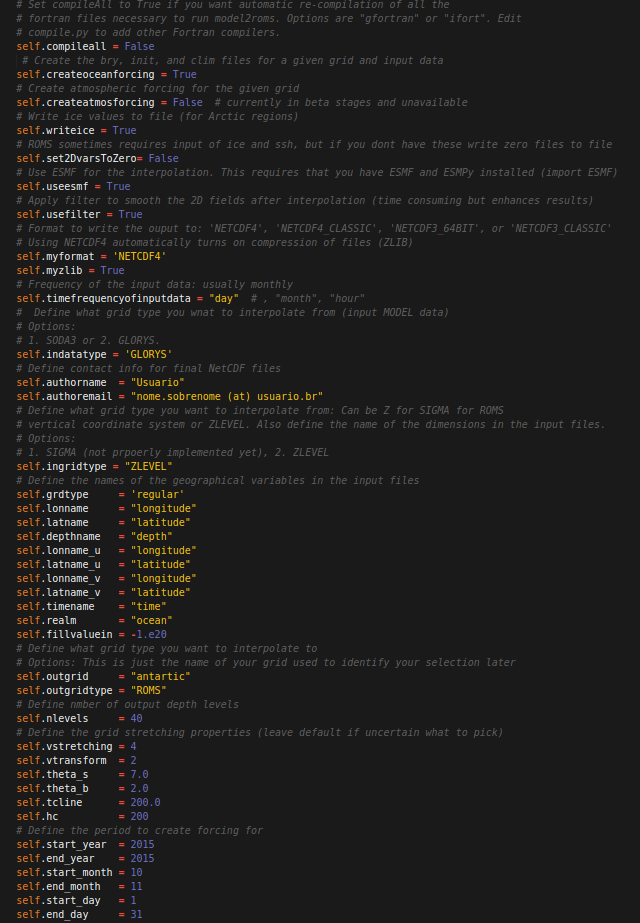
\includegraphics[width=0.5\textwidth]{m2roptions.png}
    \caption{Captura de tela do script \textit{configM2R.py}.}
    \label{m2roptions}
\end{figure}
\bigskip

\noindent Execute o \textit{model2roms} com o comando:
\bigskip

\begin{bashcode}
ipython runM2R.py
\end{bashcode}
\bigskip

\noindent Ao finalizar, serão criados os arquivos inicial, de fronteira e o climatológico.

\bigskip
   
